% From the repository root:
% latexmk -pdf -interaction=nonstopmode -halt-on-error \
%   -outdir=/tmp/fulton-harris-pilot-build docs/fulton-harris-pilot-plan.tex
% cp /tmp/fulton-harris-pilot-build/fulton-harris-pilot-plan.pdf docs/
% Companion to docs/fulton-harris-plan.tex (the whole-book plan).
\documentclass[11pt,a4paper]{article}
\usepackage[T1]{fontenc}
\usepackage{lmodern}
\usepackage[margin=22mm,headheight=15pt]{geometry}
\usepackage{amsmath,amssymb,mathtools}
\usepackage{microtype}
\usepackage[table]{xcolor}
\usepackage{booktabs,tabularx,array,longtable}
\usepackage{enumitem}
\usepackage{listings}
\usepackage{tikz}
\usetikzlibrary{arrows.meta,positioning}
\usepackage{xurl}
\usepackage{fancyhdr}
\usepackage{needspace}
\usepackage[colorlinks=true,linkcolor=teal!60!black,urlcolor=teal!60!black]{hyperref}
\definecolor{ink}{HTML}{183947}
\definecolor{muted}{HTML}{53636A}
\definecolor{pale}{HTML}{EDF4F5}
\pagestyle{fancy}
\fancyhf{}
\fancyhead[L]{\small\textcolor{ink}{Fulton--Harris pilot: detailed formalization plan}}
\fancyhead[R]{\small\textcolor{muted}{12 October 2026}}
\fancyfoot[C]{\small\thepage}
\setlength{\parindent}{0pt}
\setlength{\parskip}{5pt plus 1pt}
\setlength{\emergencystretch}{2em}
\setlist{leftmargin=*,itemsep=3pt,topsep=4pt,parsep=0pt}
\renewcommand{\arraystretch}{1.15}
\newcolumntype{P}[1]{>{\raggedright\arraybackslash}p{#1}}
\newcolumntype{Y}{>{\raggedright\arraybackslash}X}
\newcommand{\code}[1]{\texttt{\detokenize{#1}}}
\newcommand{\src}[1]{{\footnotesize\nolinkurl{#1}}}
\newcommand{\Q}{\mathbb Q}
\newcommand{\C}{\mathbb C}
\newcommand{\Hom}{\operatorname{Hom}}
\newcommand{\tr}{\operatorname{tr}}
\newcommand{\stage}[2]{\par\needspace{4\baselineskip}\textbf{#1. #2}\par}
\newcommand{\decision}[1]{\begin{center}\fcolorbox{pale}{pale}{\parbox{0.94\linewidth}{#1}}\end{center}}
\newenvironment{item-spec}[2]{\needspace{8\baselineskip}\subsection*{#1\quad #2}}{}
\newcommand{\field}[1]{\par\textbf{#1.}~}
\lstdefinelanguage{Arend}{
  morekeywords={\\func,\\lemma,\\sfunc,\\class,\\record,\\instance,\\cowith,\\where,
    \\extends,\\override,\\import,\\open,\\Pi,\\Sigma,\\lam,\\let,\\have,\\in,\\case,
    \\with,\\elim,\\new,\\Prop,\\Set,\\Type,\\property,\\field,\\use,\\level,\\protected,
    \\private,\\alias,\\infixl,\\fixl},
  sensitive=true,
  morecomment=[l]{--},
  morecomment=[n]{\{-}{-\}},
}
\lstset{language=Arend,basicstyle=\footnotesize\ttfamily,columns=fullflexible,keepspaces=true,
  keywordstyle=\color{ink}\bfseries,commentstyle=\color{muted}\itshape,
  showstringspaces=false,breaklines=true,frame=single,rulecolor=\color{pale},
  backgroundcolor=\color{pale},xleftmargin=5pt,xrightmargin=5pt,
  aboveskip=7pt,belowskip=7pt,literate={→}{{$\to$}}1 {∃}{{$\exists$}}1 {∀}{{$\forall$}}1 {∘}{{$\circ$}}1 {≅}{{$\cong$}}1 {⊗}{{$\otimes$}}1}
\hypersetup{pdftitle={Fulton--Harris pilot: detailed formalization plan},
  pdfauthor={Project planning study},pdfsubject={Representation theory, arend-lib, Lectures 1--2}}

\begin{document}
\thispagestyle{empty}
{\color{ink}\Huge Fulton--Harris pilot\\[3pt] Detailed formalization plan\par}
\vspace{3mm}
{\Large Lectures 1--2, items P01--P12, and the exact $S_3$ example\par}
\vspace{3mm}
{\color{muted}12 October 2026\quad/\quad companion to \src{docs/fulton-harris-plan.tex}\par}
\vspace{3mm}

\decision{\textbf{What this document adds.} The whole-book plan fixes the
pilot's \emph{scope}: 12 items from Lectures 1--2, the $S_3$ regression example
and a choice-free policy. This document turns that scope into work: concrete
data structures, proposed Arend signatures, a proof route for each item, the
infrastructure lemmas each route needs, a dependency-ordered schedule, and
acceptance commands. Every library name below was retrieved from the checkout
on 12 October 2026 with the rebuilt CLI (\code{-ss}, \code{-fu}, \code{-ch}).
Signatures marked \emph{sketch} are design proposals that have not been
typechecked yet.}

\section*{Summary}
\begin{itemize}
  \item \textbf{The M0 blocker is resolved for the pilot cone.} A rebuilt
  \code{cli-1.12.0-full.jar} typechecks all 447 modules. A fresh
  \code{--no-daemon -r -c} check of the six representation modules exits~0 with
  no errors (Section~\ref{sec:baseline}).
  \item \textbf{The pilot cone is axiom-free by imports.} No representation,
  linear-algebra, trace, tensor, rational, complex or symmetric-group module can
  reach \code{Logic.Classical} or \code{Logic.Choice}. In the whole library, only
  \src{Arith/Complex/FTA/Classical.ard} uses an axiom, and nothing imports it.
  \item \textbf{Replacing \code{IsIrreducible} is cheap.} Its only consumers are
  \code{SchurLemma}, which has no callers, and
  \code{PermutationRepresReducible.Not-Irreducible}. For the
  finite-dimensional pilot, the proposed notion \code{IsFinIrreducible} tests
  \emph{split} invariant subspaces, given as an inclusion with a linear
  retraction, over any \code{NonZeroRing} (Section~\ref{sec:design}, D3). It is \emph{not}
  the general replacement for arbitrary modules. That design is a separate
  item, D3b, and the name \code{IsIrreducible} is reserved for it.
  \item \textbf{The work is mostly linear-algebra infrastructure.} The library
  has bases, coordinates, matrices of maps, change of basis, Smith-form ranks,
  finiteness of kernels and images, and trace invariance under conjugation. It
  lacks basis-independent traces, block and Kronecker traces, a basis for Hom,
  bases of products and tensor products, and trace~=~rank for idempotents. The
  plan registers 22 infrastructure items, L01--L22 (L08 split into L08a and L08b)
  (Section~\ref{sec:infra}).
  \item \textbf{Decidable zero only where it is used.} The definitions are
  stated over \code{Ring}, \code{CRing} or \code{Field}. \code{DiscreteField}
  is a hypothesis only of the kernel and image constructions that test pivots:
  image splitting (L08b), Schur via kernel and image (P03), and dimension of
  invariants (P11). Averaging stays over \code{CRing} with
  \code{Monoid.Inv (natCoef card)}.
  \item \textbf{A small constructive-$\C$ bridge is in the pilot.} The explicit
  $S_3$ example is transported to \code{ComplexField} (R8a and R8b). This covers its
  matrices, decomposition maps, character values and scalar commutant, with
  explicit inverses for the denominators $2$, $3$ and $6$. Irreducibility over
  $\C$ gets its own argument, through the scalar commutant and Maschke averaging
  (L21), which needs no zero test. General scalar-extension machinery stays
  deferred.
  \item \textbf{One deliberate deviation from the book.} P07 (uniqueness of
  multiplicities) goes through characters, so it comes after P12. It assumes
  characteristic~0 through injectivity of \code{natCoef}, which holds over $\Q$,
  and it inherits the dependence of P12 on Exercise~1.2. Both are recorded: the
  relation is \code{restricted} and the status is
  \code{conditional-on-exercises}.
\end{itemize}

\newpage
\section{Baseline established on 12 October}\label{sec:baseline}
{\small
\begin{tabularx}{\linewidth}{@{}P{38mm}YP{30mm}@{}}
\toprule
Check & Result & Status vs.\ 8 Oct \\
\midrule
Rebuild & \code{./gradlew :cli:jarDep :arend-lib:meta:classes} succeeds; \code{cli/build/libs/cli-1.12.0-full.jar}; OpenJDK 21.0.10. & Was: unsuitable jar \\
Whole library & Daemon bootstrap typechecked and serialized all 447 modules in 44.7\,s with no \code{[ERROR]} (loads existing \code{.arc} where valid). & New \\
Fresh pilot cone & \code{arend --no-daemon -r -c} on \code{Irreducible}, \code{MaschkeLemma}, \code{Characters}, \code{PermutationRepresentation}, \code{Product}, \code{LinRepresCat}: exit 0, zero errors, 10.8\,s. & Was: parse failure at \code{Equiv:15:24} \\
Axioms present & \code{\axiom}s: \code{alem}, \code{achoice} (\src{Logic/Classical.ard:9,11}); \code{adchoice}, \code{acchoice} (\src{Logic/Choice.ard:6,26}). \code{alem} has no usages. & Confirmed \\
Axiom reachability & Import closure (over-approximation) of every pilot module avoids both axiom modules. Only importer of \code{Logic.Choice}: \src{Arith/Complex/FTA/Classical.ard:18}, itself unimported. & New; sound because every answer is ``no'' \\
Goal reporting & Named goals parse: \code{{?name}} and \code{{?name(e)}} (\src{Arend.g4:262}). Printed as \code{[GOAL] ... Goal name}. Goals do \emph{not} set a failing exit code; \code{-c} treats GOAL like ERROR. & New \\
Daemon caveat & A daemon fixes \code{-c}, \code{-r}, \code{--serialize}, \code{-L} at start-up and ignores per-request values. Acceptance runs must pass \code{--no-daemon}. & New \\
Tests & \code{test/} has 34 meta/solver tests and no representation tests. Negative tests use the \code{fails} meta. & Confirmed \\
\bottomrule
\end{tabularx}}

\textbf{Remaining M0 items.} (1) Run \code{arend --no-daemon -r -c} and
\code{-t -r -c} over the whole library, and record the hashes of the jar,
\code{arend-lib/ext} classes and the source tree. (2) Add the two control tests
of Section~\ref{sec:verify}. (3) Check in the import-closure audit script under
\src{tools/autoformalization/}. (4) Note one stale comment:
\src{Arith/Complex/FTA.ard:42} names a nonexistent \code{Arith.Complex.FTA.Choice}.

\section{Pilot scope and exit criteria}\label{sec:scope}
\textbf{In scope.}
\begin{itemize}
  \item P01--P12 from the whole-book plan.
  \item One extra item, P01b: an Arend proof that the old irreducibility notion
  implies excluded middle.
  \item The $S_3$ regression suite: R1--R7 over $\Q$, and R8a/R8b, the
  explicit transport of the example to constructive $\C$ (structure, then
  characters).
  \item The infrastructure L01--L22 that these need.
\end{itemize}

\textbf{Out of scope; recorded as deferred.}
\begin{itemize}
  \item General scalar-extension machinery: transfer of arbitrary theorems from
  $\Q$ to $\C$ (an M2 bridge).
  \item The general irreducibility notion for arbitrary, possibly
  infinite-dimensional, modules (D3b).
  \item The exterior-square conjunct of Prop.~2.1.
  \item A general decomposition algorithm for Cor.~1.6.
  \item Completeness of the $S_3$ character table: that the number of
  irreducibles equals the number of classes.
  \item Hermitian forms.
  \item Proofs of Exercises~1.2 and~2.5, which stay as intentional holes.
\end{itemize}

\textbf{Exit criteria.} There are two tiers, because the tensor basis (L14)
is allowed to finish after everything else.
\begin{enumerate}
  \item \textbf{Core pilot complete.}
  \begin{enumerate}
    \item Every P-, L- and R-item has a manifest record whose
    \code{statement_review} has a recorded outcome.
    \item A fresh \code{--no-daemon -r -c} run of the touched modules reports
    exactly two goals, \code{FH_L01_Ex1_2} and \code{FH_L02_Ex2_5}, and no
    unregistered goals or errors.
    \item L14 and the tensor conjunct of P09 may be absent from the source, but
    their manifest records must say \code{pending} with the reason. No goal
    may stand in for them.
    \item Every declaration outside the dependency closure of the two exercise
    goals is reported \code{checked}. Every declaration inside it is reported
    \code{conditional-on-exercises}.
    \item The axiom audit reports no path to \code{Logic.Classical} or
    \code{Logic.Choice}.
    \item The effort measurements of Section~\ref{sec:measure} are recorded.
  \end{enumerate}
  \item \textbf{All selected items complete.} The core criteria hold, and in
  addition L14 and the tensor conjunct of P09 are checked, so no item is
  \code{pending}.
\end{enumerate}
Only the second tier is reported as ``pilot complete'' without qualification.

\newpage
\section{Design decisions}\label{sec:design}

\stage{D1}{Scalars}
\begin{itemize}
  \item Group-theoretic identities (actions, traces of products, averaging) are
  stated over \code{{R : CRing}}. Averaging takes
  \code{cardInv : Monoid.Inv (R.natCoef G.card)}, matching the existing
  \code{MaschkeLemma} class.
  \item Definitions use the weakest class that makes them meaningful. The
  split subrepresentation works over any \code{Ring}, and
  \code{IsFinIrreducible} over any \code{NonZeroRing}, which excludes the zero
  ring. The Hom and dual representations need a \code{CRing}.
  \item \code{DiscreteField} is a hypothesis only of constructions that test
  pivots, that is, kernel and image bases built from \code{image-fin},
  \code{kernel-fin} and \code{smith-bases}
  (\src{Algebra/Linear/VectorSpace.ard:125--187}). These need a
  \code{SmithDomain}; \code{-ch} confirms that \code{DiscreteField} is one. See
  L08 for which of these split over a general \code{SmithDomain}.
  \item Results whose proofs avoid pivots are stated over \code{Field} or
  \code{LocalRing}, so that they apply to \code{ComplexField}. Examples are L21
  and the R8a/R8b bridge.
  \item Concrete examples use \code{RatField : DiscreteOrderedField Rat}
  (\src{Arith/Rat.ard:145}).
  \item For $|G|^{-1}$ over $\Q$, build the inverse from
  \code{RatField.nonZero-Inv} and \code{natRat/=0}
  (\src{Arith/Rat.ard:337}). This is infrastructure lemma L16.
\end{itemize}

\stage{D2}{Finite-dimensional representations: truncated versus chosen bases}
Two layers are added. The first is the interface; the second does the
computing.
\begin{lstlisting}
-- sketch; Algebra/Group/Representation/FinRepres.ard
\class FinLinRepres \extends LinRepres, FinModule     -- isFinModule : ∃ basis (truncated)

\class BasedLinRepres \extends LinRepres {            -- chosen basis, for computation
  | basis : Array E
  | isBasis : IsBasis basis
}
\func BasedLinRepres.toFin (B : BasedLinRepres) : FinLinRepres  -- forget the choice
\end{lstlisting}
Rules:
\begin{itemize}
  \item Scalars and dimensions over a \code{FinLinRepres} are defined only
  through basis-independence. This follows the \code{dimension-pair} pattern:
  a \code{\level}~\code{\Sigma} over the truncated basis
  (\src{Algebra/Module/FinModule.ard:47}).
  \item Constructions such as matrices, splittings and averaged projectors
  take a \code{BasedLinRepres}.
  \item No global choice of a basis is made anywhere.
\end{itemize}

\stage{D3}{Finite-dimensional irreducibility via split invariant subspaces (pilot notion)}
A split subrepresentation is data: a representation \code{sub}, an intertwiner
\code{incl} into $E$, and a \emph{linear} retraction of \code{incl}. The
retraction makes \code{incl} a split monomorphism (\code{SplitMono},
\src{Category.ard:61}) in the category of modules \code{LModuleCat}, not in the
category of representations \code{RepresentationCat}.
\begin{lstlisting}
-- Algebra/Group/Representation/SplitSubLRepres.ard
\record SplitSubLRepres.{u} {R : Ring.{u}} {G : Group.{u}} (E : LinRepres.{u} R G)
  | sub : LinRepres.{u} R G
  | incl : IntertwiningMap sub E
  | split : SplitMono {LModuleCat.{u} R} {sub} {E} incl

-- an invariant split submodule (R^k, incl, retr) gives sub = R^k with g . x := retr (g ** incl x)
\func SplitSubLRepres.fromInvariant (S : SplitSubLModule E P) (P-inv : ...) : SplitSubLRepres E

-- Algebra/Group/Representation/Irreducible.ard (pilot notion; no decidable equality)
\func IsFinIrreducible.{u} {R : NonZeroRing.{u}} {G : Group.{u}} (E : LinRepres.{u} R G) : \Prop
  => \Sigma (∃ (l : Array E) (0 < l.len) (E.IsBasis l))              -- finite free, positive rank
            (\Pi (S : SplitSubLRepres.{u} E) -> (\Pi (x : S.sub) -> x = 0) || IsSurj S.incl)
\end{lstlisting}
\begin{itemize}
  \item \textbf{Linear, not equivariant, retraction.} A split monomorphism in
  \code{RepresentationCat} is an invariant direct summand, and testing only
  those defines indecomposability. Over $\mathbb F_2$, the swap action of
  $C_2$ on $\mathbb F_2^2$ is indecomposable but not irreducible: the line
  spanned by $(1,1)$ is invariant and linearly split, but has no invariant
  complement. The equivariant split is what averaging produces
  (\code{maschke-split}, P04a), when $|G|$ is invertible.
  \item \textbf{Universe levels.} \code{LModuleCat} and
  \code{RepresentationCat} take objects at a finite level \code{u}, so
  \code{SplitSubLRepres}, \code{IsFinIrreducible} and the declarations that
  quantify over them carry a level parameter \code{.\{u\}}.
  \item \textbf{No decidable equality in the definition.} The first component
  is the truncated existence of a basis of positive length; no basis is
  chosen, and no \code{dimension} or decision procedure is needed. (An earlier
  version phrased it as a surjective split inclusion $R^k \to E$. That is
  equivalent, since such an inclusion is an isomorphism and its invariance
  condition is automatic, but it misleadingly looked like a statement about
  subrepresentations.)
  \item \textbf{Nontrivial scalars are required.} Positive rank alone does not
  exclude the zero module. Over the zero ring, $R^1$ is already zero, and with
  \code{{R : Ring}} the predicate would call it irreducible. Hence
  \code{{R : NonZeroRing}}. This is a nontriviality assumption, the negated
  equality $0\ne1$; it is not positive evidence in the apartness or
  invertibility sense. It needs no decidable equality. The alternative of an explicit nontriviality field on
  $E$ is listed for review. \code{DiscreteField} only enters through the constructions that
  produce split subspaces (L08b, P03).
  \item \textbf{Why this escapes the $W_P$ argument.} A split subspace comes
  with a retraction. For $W_P\subseteq\Q$ that would mean a linear
  $r:\Q\to W_P$ with $r\circ j=\mathrm{id}$, so $j\circ r$ is multiplication
  by an idempotent $c\in\Q$, and $c=0$ or $c=1$ decidably. Building that data
  already settles $P$.
  \item \textbf{Invariance is a proposition.} It is an equation in a set, so no
  data has to be chosen to state it.
  \item \textbf{Recorded restrictions.}
  \begin{itemize}
    \item The notion only makes sense for finite free representations, and it
    tests only split invariant subspaces of finite rank.
    \item It is the pilot's working definition, not the general replacement.
    Arbitrary and infinite-dimensional modules (for example Verma modules)
    need the separate design item D3b, which is out of scope here.
    \item The name \code{IsIrreducible} stays unassigned until D3b is decided.
  \end{itemize}
  \item \textbf{Open questions for M1 review.}
  \begin{itemize}
    \item Should a nonzero-vector witness replace the positive-rank component?
    \item \code{sub} is an arbitrary representation, so finite projective
    summands are allowed. Rank-one irreducibility then needs a ring without
    nontrivial idempotents: over $R\times R$, the summand $R\times 0$ is a
    split subrepresentation. Is this the right generality for D3b?
  \end{itemize}
  \item \textbf{The old definition.} It is renamed
  \code{IsStronglyIrreducible} and kept together with its Schur proof, so that
  P01b can state the excluded-middle consequence. The doc comment says the
  notion is classical-strength and must not be used as a default.
\end{itemize}

\stage{D4}{Representations built from others}
\begin{lstlisting}
-- sketch; Algebra/Group/Representation/Hom.ard
\func HomLRepres {R : CRing} {G : Group} (A B : LinRepres R G) : LinRepres R G
  -- carrier LinearMapLModule A B;  (g . phi) v = g ** phi (inverse g ** v)
\func DualLRepres {R : CRing} {G : Group} (A : LinRepres R G) : LinRepres R G
  => HomLRepres A (TrivialAction (RingLModule R) G)
-- Algebra/Group/Representation/Tensor.ard
\func TensorLRepres {R : CRing} {G : Group} (A B : LinRepres R G) : LinRepres R G
  -- carrier TensorProductModule A B; g acts by tensorLift of (a, b) |-> g a ⊗ g b
\end{lstlisting}
\begin{itemize}
  \item The direct sum is the existing \code{ProductLRepres}.
  \item Finite indexed sums are iterated \code{ProductLRepres}. They are only
  needed in the $S_3$ example and in P07, both with a small fixed number of
  summands.
  \item The library's misspelled \code{InterwiningMap} (and the module of that
  name) was renamed to \code{IntertwiningMap}, overriding the whole-book plan's
  instruction to keep the existing spelling.
\end{itemize}

\stage{D5}{Characters}
\begin{itemize}
  \item The existing \code{Character E bv g} becomes the \emph{based}
  character.
  \item The basis-free \code{character} on a \code{FinLinRepres} is defined
  by eliminating the truncated basis into a level-$(-1)$
  $\Sigma$-type, as \code{dimension-pair} does. This needs L05.
  \item Class functions are \code{G -> R} with
  \code{\Pi g h -> f (h * g * inverse h) = f g}.
  \item The pairing is the inverse-character one:
  $\langle\chi,\psi\rangle = |G|^{-1}\sum_g\chi(g^{-1})\psi(g)$.
  \item Comparing with the book's conjugate pairing belongs to the deferred
  $\C$ bridge.
\end{itemize}

\stage{D6}{Exercise holes}
Exercises 1.2 and 2.5 are stated in full. Their bodies are the named goals
\code{{?FH_L01_Ex1_2}} and \code{{?FH_L02_Ex2_5}}, and each declaration's doc
comment cites the exercise. Consumers are written against the statement and
inherit \code{conditional-on-exercises}.
\begin{itemize}
  \item \textbf{To be checked in M0.} The checker must still elaborate a
  consumer whose dependency has a goal body.
  \item \textbf{Fallback.} If it cannot, the consumer takes the exercise
  statement as an explicit hypothesis. Its name gets the suffix
  \code{-cond}; for example, the conditional form of
  \code{orthogonality} is \code{orthogonality-cond}.
\end{itemize}

\stage{D7}{Placement and names}
New declarations go in mathematical modules under
\src{Algebra/Group/Representation/} and \src{Algebra/Module/}, and they follow
the naming table of the \code{arend-formalize} skill. Book numbers appear only
in doc comments (\code{-- | Fulton--Harris Prop.~1.5}) and in the manifest.
The $S_3$ objects that are reusable (the sign representation and the standard
representation of $S_n$ for $n=3$) go in the library. The $S_3$ numerical
checks go in \src{test/Algebra/Representation/S3Test.ard}.

\newpage
\section{Infrastructure backlog}\label{sec:infra}
Each L-item is a lemma or construction missing from the checkout. Its absence
was confirmed by symbol search, usages and signature search. Sizes are rough
proof-effort classes: S is under 30 lines, M is 30--150, L is over 150.

{\small
\begin{longtable}{@{}P{9mm}P{55mm}P{50mm}P{8mm}P{24mm}@{}}
\toprule
ID & Statement (sketch) & Reuse & Size & Consumers \\
\midrule
\endhead
L01 & \code{toLinearMap_*}: \code{E.toLinearMap (g * h) = E.toLinearMap g} $\circ$ \code{E.toLinearMap h} & \code{**-assoc}, \code{exts} & S & L05, P08, P11 \\
L02 & Matrices of the action reverse products: \code{toMatrix lv bv (toLinearMap (g*h)) = toMatrix .. h product toMatrix .. g}. So $g\mapsto$ matrix of $\rho(g)$ is an \emph{anti}homomorphism into \code{MatrixRing}; the homomorphism is $g\mapsto$ matrix of $\rho(g^{-1})$, or a map from the opposite group & L01, \code{toMatrix_*} (\src{LinearMap.ard:109}; row convention) & S & P01, P08, P09 \\
L03 & \code{toMatrix} is linear in the map: \code{toMatrix_+}, \code{toMatrix_*c}, \code{toMatrix_BigSum}, \code{toMatrix_FinSum} & \code{basis-split-unique}, \code{linearMap_BigSum} & M & P11 \\
L04 & Trace is basis independent: \code{Trace (toMatrix lu bu f) = Trace (toMatrix lu' bu' f)} for an endomorphism & \code{change-basis_matrix-left}, \code{-right}, \code{toMatrixInv}, \code{basis-iso}, \code{Trace-conjugation} or \code{Trace-prod} & M & L05 \\
L05 & \code{endoTrace {R : NonZeroCRing} (U : FinModule R) (f : LinearMap U U) : R}, defined by the \code{dimension-pair} pattern, with \code{endoTrace-char} & L04 & S & P08, P11 \\
L06 & Trace of a block-diagonal matrix: \code{Trace (blockMatrix A B) = Trace A + Trace B} & \code{blockMatrix}, \code{elem00/11} (\src{Matrix.ard:51}) & S & P09 \\
L07 & Basis of \code{ProductLModule}: \code{in1}-images followed by \code{in2}-images; matrix of a product map is \code{blockMatrix} & \code{IsBasis}, \code{basis-split-unique} & M & P09 \\
L08a & \textbf{Kernel splits over a \code{SmithDomain}.} With \code{smith-bases}, $f(u'_j)=d_jv'_j$, and $\ker f$ is spanned by the $u'_j$ with $d_j=0$, because a \code{SmithDomain} is a domain and $d_j=0$ is decidable. Projection onto those coordinates is a retraction. & \code{smith-bases}, \code{kernel-fin} & M & P03, P04b \\
L08b & \textbf{Image splits only with invertible pivots.} Over a general \code{SmithDomain} it fails: $2\cdot{}:\mathbb Z\to\mathbb Z$ has image $2\mathbb Z$, which has a basis but no retraction from $\mathbb Z$. So the image of $f$ is split if every nonzero Smith coefficient $d_j$ is invertible; this holds automatically over a \code{DiscreteField}. The retraction sends $v'_j\mapsto d_j^{-1}e_j$ for $j<\mathrm{rank}$. & \code{smith-bases}, \code{image-fin} & M & P03 \\
L09 & Over a \code{DiscreteField}: \code{retr} $\circ$ \code{incl = id} and \code{dim = T.dim} (a full split subspace) imply \code{IsSurj incl} & \code{toMatrix_*}, \code{matirx-inv} (sic, \src{Matrix.ard:542}), \code{matrix-split_<=} & S & P03 \\
L10 & Dimension bound: a split inclusion has \code{dim <= T.dim} over a \code{NonZeroCRing} & \code{matrix-split_<=} (\src{Matrix.ard:645}) & S & L21, R3 \\
L11 & Basis of \code{LinearMapLModule U V} for based $U,V$: matrix units; upgrade \code{matrix-equiv} (set-level, \src{LinearMap.ard:134}) to a \code{ModuleIso} & L03 & M & P02, P12 \\
L12 & Kronecker product of matrices and \code{Trace (kron A B) = Trace A * Trace B} & \code{BigSum} double-sum lemmas & M & P09, P12 \\
L13 & Matrix of $\varphi\mapsto b\circ\varphi\circ a$ in the matrix-unit basis is \code{kron (transpose A) B} & L11, L12, \code{Trace-transpose} & M & P12 \\
L14 & Basis of \code{TensorProductModule} of based modules ($e_i\otimes f_j$); tensor of linear maps; matrix is a Kronecker product & \code{tensorLift}, \code{tensorLift-unique} & L & P09 \\
L15 & Trace of an idempotent: for $p\circ p=p$ on a based module over \code{DiscreteField}, \code{endoTrace p = natCoef (dimension (image-fin p))} & L08, L07, \code{image-fin.dimension_rank} & M & P11 \\
L16 & \code{Inv (RatField.natCoef (suc n))}; injectivity of \code{natCoef} over \code{RatField} & \code{nonZero-Inv}, \code{natRat/=0} & S & P04, P07, R* \\
L17 & \code{SymFinGroup (n : Nat) : FinGroup (Sym n)} from \code{SymmetricGroup} and \code{SymFin} (no instance exists today); check that the \code{DecSet} fields agree and that \code{EquivFin} does not win instance search & \src{Algebra/Group/Symmetric.ard:65,284,297} & S & R1--R7 \\
L18 & Natural action \code{SymAction n : GSet (SymmetricGroup n)} on \code{Fin n}. Products are left-to-right (\code{(e * e') j = e' (e j)}, \src{Equiv.ard:233}), so the action must be \code{e ** i = inverse e i}; then \code{PermRepr} gives $(g\cdot f)(j)=f(g\,j)$ & \code{symQEquiv}, \code{Sym.equals} & S & R2, R4, R5 \\
L19 & Fixed points as a decidable subset of a finite \code{GSet} with decidable equality, with a \code{FinSet} instance (\code{SigmaFin.DecSubSet-isFin}); conjugacy classes of an explicit finite group as decidable subsets & \code{DecSubSet}, \code{SigmaFin}, \code{FinSum-inj} & S & P10, R1 \\
L20 & Inversion $g\mapsto g^{-1}$ as a \code{QEquiv} for every \code{Group}, and the reindexing \code{FinSum (x o inverse) = FinSum x} (today only \code{SymmetricGroup.inv-isEquiv} exists) & \code{inverse-isInv}, \code{FinSum_Equiv} & S & P09, P11, P12 \\
L21 & \textbf{Irreducibility from a scalar commutant.} Over a commutative \code{LocalRing} $R$ (hence \code{NonZeroRing}), with \code{cardInv}: if $E\cong R^n$ with $n>0$ (a full split subspace $T$ with \code{0 < T.dim}) and every intertwiner $E\to E$ is scalar, then \code{IsFinIrreducible E}. Positive rank is essential, since the zero representation also has only scalar endomorphisms. Route: a split invariant $S$ gives the equivariant idempotent $\pi=\mathit{incl}\circ\rho$ (P04a). By the commutant $\pi=c\cdot\mathrm{id}_E$, so $(c^2-c)\,\mathrm{id}_E=0$. Evaluating at $T.\mathit{incl}(e_0)$ and applying $T.\mathit{retr}$ gives $(c^2-c)e_0=0$ in $R^n$, hence $c^2=c$; this step uses $n>0$. Then \code{LocalRing.connected} (\src{Algebra/Ring/Local.ard:37}) gives $c=0$ (so \code{dim = 0}, using $0\ne1$) or $c=1$ (so \code{incl} is surjective). No zero test is used, so it applies to \code{ComplexField}. & P04a, \code{LocalRing.connected}, L10 & M & R3, R8a \\
L22 & Ring homomorphism $\Q\to\C$: \code{fromRealRingHom} (\src{Arith/Complex.ard:108}) composed with the structure map of \code{RealField : OrderedFieldAlgebra RatField Real}; transport of matrices (\code{matrix-map}), of traces, and of \code{Monoid.Inv} along a ring homomorphism, which gives the inverses of $2,3,6$ in \code{ComplexField} & \code{fromRealRingHom}, \code{RingHom}, \code{charPoly_map} pattern & S & R8a, R8b \\
\bottomrule
\end{longtable}}

\textbf{Notes.}
\begin{itemize}
  \item L14 is the largest item. The pilot needs the tensor character formula,
  so L14 is scheduled early, in wave~1, as an independent track. If it
  stalls, only the tensor conjunct of P09 is held up; P12 uses the Hom route
  (L11--L13) instead.
  \item For L14, \src{Algebra/Algebra/TensorProduct.ard} builds a bilinear
  multiplication by nesting \code{tensorLift}. That is the template for the
  tensor $f\otimes g$ of two linear maps. Note that \code{tensorLift_tensor} is
  propositional, not \code{idp}.
  \item L03 can reuse \code{AddMonoidHom.func-FinSum}
  (\src{Algebra/Monoid/MonoidHom.ard:92}), which applies to linear maps.
  \item L08 is the design-critical item, and it is split in two because the
  image half is false over a general \code{SmithDomain} (the counterexample
  $2\mathbb Z\subseteq\mathbb Z$ is in L08b). It is prototyped and typechecked
  first, together with D3 and P03.
  \item The image of an \emph{idempotent} is always split, with $\pi$ itself as
  the retraction onto its image. So P04, P11 and L21 never need L08b.
\end{itemize}

\newpage
\section{Item specifications}\label{sec:items}
Each item lists the source statement, the constructive target, the relation to
the source (\code{same}, \code{reformulated}, \code{restricted}), the proposed
declarations, the proof route, dependencies and acceptance. Page numbers are
printed pages; the physical PDF page is the printed page plus~15, an offset
checked on pp.~3--16.

\begin{item-spec}{P01}{Representations, based finite representations, split subobjects, irreducibility}
\field{Source} §1.1, pp.~3--4. A representation is a homomorphism
$\rho:G\to\mathrm{GL}(V)$. $V$ is irreducible if it has no proper nonzero
invariant subspace.
\field{Target}
\begin{itemize}
  \item D2 (\code{FinLinRepres} and \code{BasedLinRepres}).
  \item D3 (\code{SplitSubLRepres} and the pilot notion \code{IsFinIrreducible}).
  \item The bridge to $G\to\mathrm{GL}(V)$, with the order fixed.
  \code{LinearMapRing} multiplies as \code{f * g = g ∘ f}
  (\src{Algebra/Module/Instances.ard:28}), while an action satisfies
  $\rho(gh)=\rho(g)\circ\rho(h)$ (L01). So $g\mapsto\rho(g)$ is an
  \emph{anti}homomorphism into the units of \code{LinearMapRing E}. The bridge
  is therefore \code{LinRepres.toGroupHom : GroupHom G (units of LinearMapRing E)}
  with $g\mapsto\rho(g^{-1})$. The equivalent alternative, a homomorphism from
  the opposite group with $g\mapsto\rho(g)$, is recorded for review. Either
  way, the construction comes with its inverse.
\end{itemize}
Relation: \code{reformulated}. Invariant subspaces are replaced by split ones.
\field{Route}
\begin{itemize}
  \item The induced action on $R^{\mathit{dim}}$ is
  $g\cdot x=\mathit{retr}(g\cdot\mathit{incl}\,x)$.
  \item Its \code{**-assoc} uses \code{incl-invariant} and \code{retr_incl}.
  \item The bridge reuses \code{toLinearMap}, \code{toLinearMap_ide}, L01 and
  \code{inverse_*}. A regression test pins the direction of the homomorphism.
\end{itemize}
\field{Migration}
\begin{itemize}
  \item Restate \code{PermutationRepresReducible.Not-Irreducible}
  (\src{PermutationRepresentation.ard:57--67}) for the new notion, over an
  arbitrary ring and an arbitrary \code{GSet X}, with the same hypotheses as
  now. The old theorem's conclusion \code{0 = {R} 1} turns into the hypothesis
  that $R$ is a \code{NonZeroRing}, and the new conclusion is
  \code{Not (IsFinIrreducible (PermRepr X))}.
  \item The constant line $j(c)=(c,c,\dots)$ with $r(f)=f(x_0)$ is a
  split invariant subspace of dimension~1 for any $X$. \code{nonConstantVector}
  shows that $j$ is not surjective. The refutation only uses the second
  component of \code{IsFinIrreducible}.
  \item \textbf{Recorded change of strength.} For infinite $X$, the new
  predicate's first component, finite freeness, generally fails anyway.
  The migrated theorem is then weaker than the old one, which refuted
  irreducibility in the strong sense for every $X$. The general-module form
  waits for D3b.
  \item \code{SubLRepres.IsTrivial} stays, documented as the strong
  dichotomy.
\end{itemize}
\field{Acceptance} One-dimensional examples are irreducible over any
\code{NonZeroCRing}: the trivial and sign representations (L10 gives
$\mathit{dim}\le1$). The migrated \code{Not-Irreducible} checks.
\end{item-spec}

\begin{item-spec}{P01b}{The old notion implies excluded middle}
\field{Target} \code{IsStronglyIrreducible.excludedMiddle}: from
\code{IsStronglyIrreducible (TrivialAction (RingLModule R) G)} and $0\neq1$
in $R$, derive \code{\Pi (P : \Prop) -> P || Not P}.
\field{Route}
\begin{itemize}
  \item The submodule is $W_P$ with \code{contains x => P || x = 0}. Its
  closure fields are short case splits.
  \item Then follow the two cases of the whole-book plan, page~4.
  \item This is an ordinary constructive theorem. It introduces no axiom and
  documents why D3 is needed.
\end{itemize}
\field{Size} S. It is a good first task for calibrating the workflow.
\end{item-spec}

\begin{item-spec}{P02}{Direct sum, dual and Hom representations; Exercise 1.2 (hole)}
\field{Source} §1.1, pp.~4--5; Exercise~1.2.
\field{Target} \code{HomLRepres} and \code{DualLRepres} (D4); the existing
\code{ProductLRepres}. Exercise 1.2 as an intentional hole:
\begin{lstlisting}
-- | Fulton--Harris Exercise 1.2: invariant vectors of Hom(V, W) are the G-linear maps.
\lemma invariantHom {R : CRing} {G : Group} {A B : LinRepres R G} (f : LinearMap A B)
  : (\Pi (g : G) -> g HomLRepres.** f = f) <-> (\Pi (g : G) (a : A) -> f (g ** a) = g ** f a)
  => {?FH_L01_Ex1_2}
\end{lstlisting}
Relation: \code{same}.
\field{Route} The action fields of \code{HomLRepres} are pointwise, using
\code{exts}, \code{**-assoc} and \code{inverse_*}. The pattern to follow is
\code{IntertwiningMapLModule} in \src{LinRepresCat.ard}.
\field{Acceptance} \code{HomLRepres} and \code{DualLRepres} check, and only the
registered goal remains.
\end{item-spec}

\begin{item-spec}{P03}{Schur's lemma (1)}
\field{Source} Schur 1.7(1), p.~7.
\field{Target}
\begin{lstlisting}
\lemma SchurLemma {K : DiscreteField} {G : Group} {A B : BasedLinRepres K G}
  (p : IsFinIrreducible A) (q : IsFinIrreducible B) (f : IntertwiningMap A B)
  : f.IsZero || IsEquiv f
\end{lstlisting}
Relation: \code{reformulated}. It uses the pilot irreducibility. As
implemented in wave~1 it concludes \code{IsEquiv f}, like the old lemma, rather
than \code{ModuleIso}; \code{ModuleIso.iso<->inj+surj} converts between the two. The
\code{DiscreteField} hypothesis is needed for the image splitting (L08b), not
for the definitions.
\field{Route}
\begin{itemize}
  \item The kernel of $f$ is split by L08a, which works over any
  \code{SmithDomain}. The image is split by L08b, which needs invertible
  pivots, so this is where \code{DiscreteField} is used. The target is a
  proposition, so the truncation in \code{smith-bases} can be eliminated.
  \item Invariance comes from \code{KernelLRepres} and \code{ImageLRepres}.
  \item Then copy the case structure of the existing \code{SchurLemma}
  (\src{Irreducible.ard:14--21}), using L09 for ``dim equal implies surjective''.
\end{itemize}
\field{Risk} This item validates D3, so it is prototyped first, typechecked
together with L08a and L08b. If the image splitting cannot be stated cleanly,
revise D3 before writing anything else.
\field{Not covered} Schur over constructive $\C$. Specific complex maps can
have explicitly known kernel and image bases. What is missing is a general
procedure that constructs such bases, and their retractions, without
additional evidence such as invertible pivots. So the $\C$ side of the pilot
uses L21 instead.
\end{item-spec}

\begin{item-spec}{P04}{Maschke: invariant complements}
\field{Source} Prop.~1.5, p.~6.
\field{Target} Two declarations.
\begin{itemize}
  \item \code{P04a} over \code{CRing}, with $|G|^{-1}$. Given a split
  invariant subspace $S$, it returns an equivariant idempotent
  $\pi=\mathit{incl}\circ\rho$, where $\rho$ is the averaged retraction, with
  $\pi\circ\mathit{incl}=\mathit{incl}$. Its image is $S$, and it needs no basis
  and no zero test, so it also applies to \code{ComplexField}. L21 uses it.
  \item \code{P04b} over \code{DiscreteField}. It returns a complement
  $S'$ as a \code{SplitSubLRepres} together with an isomorphism of
  representations $E\cong S\oplus S'$.
\end{itemize}
Relation: \code{restricted}. The input is split rather than an arbitrary
subspace; the whole-book plan, page~6, explains why.
\field{Route}
\begin{itemize}
  \item Average $p_0=\mathit{incl}\circ\mathit{retr}$. Reuse
  \code{SumOverGroup}, \code{FinSumRewrite} and the
  \code{mean-func-preserve} argument (\src{MaschkeLemma.ard:28--45}),
  generalized from a \code{SubLRepres} target to \code{E}.
  \item The complement is $\ker\pi$, split by $\mathrm{id}-\pi$. L08a supplies
  its basis over any \code{SmithDomain}; \code{DiscreteField} is stated for
  uniformity with P03, and weakening it is a review experiment.
  \item The isomorphism is \code{coprod-map} of the two inclusions, with
  inverse $(\pi,\mathrm{id}-\pi)$.
\end{itemize}
\field{Regression} Characteristic $p\mid|G|$: over \code{FinField} with $p=2$ and
$G=S_3$, \code{cardInv} is unavailable. A test documents that the
hypothesis is needed.
\end{item-spec}

\begin{item-spec}{P05}{Complete reducibility for the presented inputs}
\field{Source} Cor.~1.6, p.~6.
\field{Target} An explicit decomposition of the permutation representation
of $S_3$ on $\Q^3$ as the trivial line plus the standard representation. It is
an isomorphism of representations with both summands proved irreducible.
Relation: \code{restricted}; the general corollary is deferred.
\field{Route} Apply P04b to the split line $(1,1,1)$, or write both
inclusions out explicitly. Irreducibility of the standard representation is R3.
\end{item-spec}

\begin{item-spec}{P06}{Schur's lemma (2): scalar commutants}
\field{Source} Schur 1.7(2), p.~7.
\field{Target}
\begin{itemize}
  \item \code{IsSplitIrreducible E}: \code{IsFinIrreducible} plus
  ``every \code{IntertwiningMap E E} is a scalar multiple of the identity''.
  \item A proof that one-dimensional representations are split irreducible.
  \item A proof that the standard representation of $S_3$ is split
  irreducible over any commutative \code{LocalRing} in which $6$ is invertible;
  L21 needs that inverse anyway. A $2\times2$ matrix commuting with $\rho(12)$
  and $\rho(123)$ is scalar, by solving linear equations. Every division is
  meant to be by a divisor of $6$; confirm this when the equations are written
  out. The representation has rank $2>0$, which L21 requires.
  Irreducibility then follows from L21. Instantiate at \code{RatField} (R7) and
  at \code{ComplexField} (R8a).
\end{itemize}
Relation: \code{restricted}. The book's eigenvalue argument needs $\C$ to be
algebraically closed. Here the scalar commutant is proved per example; the
general version is the M2 bridge.
\end{item-spec}

\begin{item-spec}{P07}{Uniqueness of multiplicities}
\field{Source} Prop.~1.8, p.~7.
\field{Target} Take pairwise non-isomorphic split irreducibles $V_i$ and two
decompositions $V\cong\bigoplus V_i^{a_i}\cong\bigoplus V_i^{b_i}$, given as
iterated \code{ProductLRepres}. Then $a=b$. Relation: \code{restricted}; it
assumes characteristic~0 through injectivity of \code{natCoef} (L16).
\field{Route (deviation)}
\begin{itemize}
  \item Characters are additive (P09) and the irreducible characters are
  orthonormal (P12). Together these give
  $\langle\chi_{V_i},\chi_V\rangle=a_i=b_i$ in $K$; L16 then gives equality
  in $\mathbb N$.
  \item The book's route, through Hom-dimensions, needs additivity of
  $\dim\Hom_G$ over direct sums. The character route reuses work the pilot
  does anyway.
\end{itemize}
Dependencies: P09, P12, L16. Through P12, P07 depends on the Exercise~1.2
hole, so its status is \code{conditional-on-exercises} until that hole is
closed; the characteristic-0 restriction appears in its signature.
\end{item-spec}

\begin{item-spec}{P08}{Basis-independent character; class function; $\chi(1)=\dim$}
\field{Source} §2.1, p.~13.
\field{Target}
\begin{itemize}
  \item \code{character (E : FinLinRepres R G) : G -> R}, defined through L05.
  \item \code{character-char}: it equals \code{Character E bv} for every basis.
  \item \code{character_conj}: \code{character E (h * g * inverse h) = character E g}.
  \item \code{character_ide}: the value at $1$ is \code{natCoef (dimension E)}.
\end{itemize}
Relation: \code{same}.
\field{Route}
\begin{itemize}
  \item Class invariance: L02 followed by \code{Trace-prod}.
  \item The value at $1$: \code{Character.of-1} (existing) and
  \code{dimension-unique}.
\end{itemize}
\end{item-spec}

\begin{item-spec}{P09}{Characters of sums, tensors and duals}
\field{Source} Prop.~2.1, p.~13.
\field{Target}
\begin{itemize}
  \item $\chi_{V\oplus W}=\chi_V+\chi_W$, using L06 and L07.
  \item $\chi_{V\otimes W}=\chi_V\chi_W$, using L12 and L14.
  \item $\chi_{V^*}(g)=\chi_V(g^{-1})$ and
  $\chi_{\Hom(V,W)}(g)=\chi_V(g^{-1})\chi_W(g)$, using L11, L13 and
  \code{Trace-transpose}.
\end{itemize}
The exterior-square conjunct is a registered pending item, not a hole.
Relation: \code{reformulated} for the dual. The book writes
$\overline{\chi_V}$; over $\C$ this agrees with $\chi_V(g^{-1})$ only after the
roots-of-unity argument, which is deferred.
\end{item-spec}

\begin{item-spec}{P10}{Permutation characters count fixed points; Exercise 2.5 (hole)}
\field{Target}
\begin{lstlisting}
-- | Fulton--Harris Exercise 2.5 (the original fixed-point formula).
\lemma permCharacter {R : CRing} {G : Group} (X : FinGSet G) (g : G)
  : Character (PermRepr X) (deltaBasis X) g
      = R.natCoef (FinSet.card (FixedPointsFin X g))
  => {?FH_L02_Ex2_5}
\end{lstlisting}
\begin{itemize}
  \item The supporting definitions are \code{deltaBasis} (the indicator
  functions) and \code{FixedPointsFin} (the decidable subset).
  \item Both definitions are proved. Only the formula itself is the hole.
\end{itemize}
Relation: \code{same}. Consumers are R5 and the character of the regular
representation (M2).
\end{item-spec}

\begin{item-spec}{P11}{Averaging onto invariants; $\dim V^G$ as a trace}
\field{Source} Prop.~2.8 and (2.9), pp.~15--16.
\field{Target}
\begin{itemize}
  \item \code{averageMap} $\varphi=|G|^{-1}\sum_g\rho(g)$, over \code{CRing}.
  \item $\varphi$ is equivariant and idempotent, and its image is exactly the
  set of invariant vectors.
  \item Over \code{DiscreteField}: \code{natCoef (dimension (invariants E))}
  equals $|G|^{-1}\sum_g\chi_E(g)$.
\end{itemize}
Relation: \code{same} for Prop.~2.8. For (2.9) it is \code{reformulated}: the
equation holds in $K$, and equality of natural numbers needs L16.
\field{Route}
\begin{itemize}
  \item Use the \code{FinSum} of \code{toLinearMap g} in \code{LinearMapAbGroup},
  reindexed with \code{FinSum_Equiv} and \code{Group.translate-is-Equiv}.
  \item Trace commutes with the sum by L03 and the linearity of
  \code{Trace}.
  \item Dimension equals trace by L15.
\end{itemize}
\end{item-spec}

\begin{item-spec}{P12}{Orthogonality of split irreducible characters}
\field{Source} Thm.~2.12 and (2.10), p.~16.
\field{Target} Two declarations, for split irreducibles $V,W$:
\begin{itemize}
  \item \code{orthogonality-iso}: from \code{ModuleIso} intertwining $V\cong W$,
  conclude $\langle\chi_V,\chi_W\rangle=1$.
  \item \code{orthogonality-noniso}: from \code{Not} (such an isomorphism),
  conclude $\langle\chi_V,\chi_W\rangle=0$.
\end{itemize}
Relation: \code{restricted}. The input is split irreducibles, and the
conclusion splits into two cases rather than a decided dichotomy.
\field{Route}
\begin{itemize}
  \item Apply P11 to \code{HomLRepres V W}. The invariants are the
  intertwiners by Exercise~1.2 (hole), so this item is
  \code{conditional-on-exercises}.
  \item In the non-isomorphic case, P03 forces every intertwiner to be zero,
  so the dimension is $0$.
  \item In the isomorphic case, P06 gives the intertwiners a basis
  $\{\mathrm{id}\}$, transported along the isomorphism, so the dimension is $1$.
  \item The character of \code{HomLRepres} comes from P09.
\end{itemize}
\end{item-spec}

\newpage
\section{The exact \texorpdfstring{$S_3$}{S3} regression suite}\label{sec:s3}
All objects are stated over an abstract commutative ring or \code{LocalRing}
and instantiated at \code{RatField} and at \code{ComplexField}. The group is
$G=$ \code{SymFinGroup 3} (L17). The
generators are $\sigma=(1\,2)$ (\code{transposition}) and $\tau=(1\,2\,3)$
(\code{cycle}, \src{Symmetric.ard:139}). The sign is \code{signHom}
(\src{Symmetric.ard:574}).

{\small
\begin{tabularx}{\linewidth}{@{}P{9mm}YP{42mm}@{}}
\toprule
ID & Statement & Route \\
\midrule
R1 & The six elements, listed explicitly, are pairwise distinct and exhaust $S_3$. The class sizes are $1,3,2$; each class is a decidable subset with its \code{card} computed. \code{card = fac 3} reduces to $6$. & L17, L19; decidable equality from \code{SymFin}; \code{Sym.equals} \\
R2 & Representations: trivial; sign ($g\cdot x=\mathrm{sgn}(g)x$, a new \code{CharacterLRepres} for a \code{MonoidHom} into the multiplicative monoid, using \code{signHom} and \code{sign_*}); \code{PermRepr} on \code{Fin 3}; standard ($e_1-e_2$, $e_2-e_3$, as a \code{SplitSubLRepres} of \code{PermRepr}). The standard representation is given by an explicit inclusion $R^2\to R^3$ and an explicit retraction, so it needs only the D3 definitions (wave 1), not the P01 bridge or the product basis L07. & D3, L18 \\
R3 & The standard representation is irreducible, by L21 applied to the scalar commutant (R7). A split invariant subspace gives an equivariant idempotent (P04a), which is a scalar $c$ with $c^2=c$, so $c=0$ or $c=1$ by locality. The same proof works over \code{ComplexField} (R8a). \emph{Rejected route:} excluding a rational eigenvector of $\tau$ needs a proof that $\lambda^2+\lambda+1$ has no rational root, for example by ordered-field positivity; \code{equation.cRing} alone cannot do it, and the route does not transfer to $\C$. & R7, L21, P04a \\
R4 & \code{PermRepr} is isomorphic to trivial $\oplus$ standard (P05). & P04b or explicit maps \\
R5 & Character rows: trivial $(1,1,1)$, sign $(1,-1,1)$, standard $(2,0,-1)$ on $[1],[\sigma],[\tau]$; permutation $(3,1,0)$, also as P10's consequence (conditional). & Explicit $2\times2$ traces \\
R6 & Orthogonality table: the nine pairings $\langle\chi_i,\chi_j\rangle$ computed by exact arithmetic with weights $1,3,2$ and $|G|^{-1}=1/6$. & L16, normalization in \code{Rat} \\
R7 & Scalar commutant of the standard representation over a commutative \code{LocalRing} with $6$ invertible (P06), instantiated at \code{RatField}; and the Hom-dimension consequences used in P12. Proved before R3 and R8a, which depend on it. & Linear equations over an abstract ring \\
R8a & \textbf{Constructive-$\C$ bridge, structural stage.} Transport R2's matrices along the ring homomorphism $\Q\to\C$ (L22). This gives the decomposition maps of R4, with their inverses, and $|G|^{-1}$ and the other denominators as images of rational inverses, so no zero test on $\C$ is used. The scalar commutant of R7 is instantiated at \code{ComplexField}. Irreducibility over $\C$ gets its own proof through L21; it is \emph{not} inferred from irreducibility over $\Q$, since irreducibility does not transfer in general. & L21, L22, P04a, R4, R7 \\
R8b & \textbf{Constructive-$\C$ bridge, character stage.} The character values of R5 over \code{ComplexField}, as images of rationals under L22 (traces commute with ring homomorphisms), and the R6 pairings over $\C$. & R5, R6, R8a, L22 \\
\bottomrule
\end{tabularx}}

\textbf{Arithmetic risk; abstract-then-instantiate is mandatory.}
\begin{itemize}
  \item \code{Rat} values are normalized by gcd, so closed \code{Rat}
  identities may not reduce to \code{idp}.
  \item Concrete \code{Complex} arithmetic unfolds into \code{re}/\code{im}
  components. \code{equation.cRing} then fails even on \code{x * y = y * x}, and
  \code{rewrite} cannot match under \code{*} (failure mode~16 of the
  \code{arend-prove} skill).
  \item Therefore R2--R8b are stated and proved over an abstract
  \code{{R : CRing}} or \code{LocalRing}, with explicit inverses of the needed
  integers as parameters. They are then instantiated twice, at \code{RatField}
  and at \code{ComplexField}.
  \item Concrete-field proofs are limited to supplying those inverses (L16,
  L22) and to the instantiation step.
\end{itemize}

\newpage
\section{Dependency order and schedule}\label{sec:order}
The work runs in waves. Items inside a wave are \emph{not} all independent:
each wave lists its items as chains, written $a\to b$, and $a\mid b$ separates
items that can run in parallel. An item may only start once everything before
it in its chain, and every earlier wave it depends on, has checked.

The recommended start is a typechecked prototype of D3, L08 and Schur (wave~1).
Wave~2 then tests the interfaces on the $S_3$ decomposition and scalar
commutant, over both $\Q$ and constructive $\C$, before the general character
theory is built.

\begin{center}
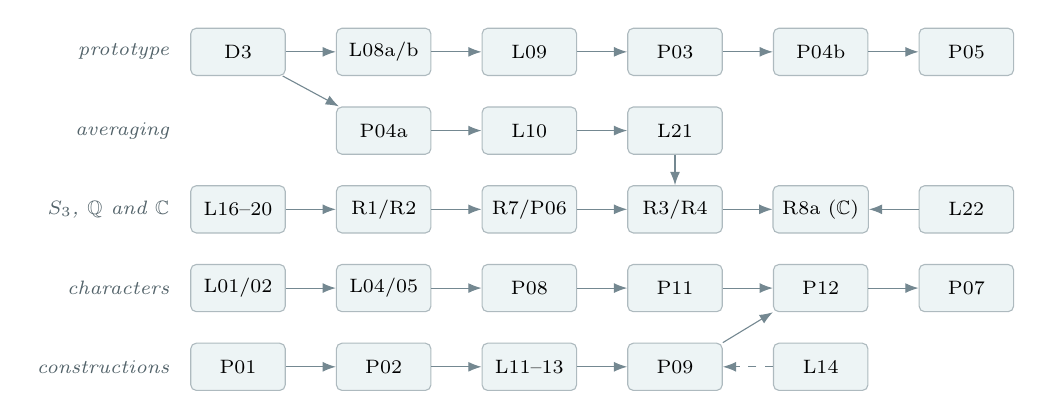
\begin{tikzpicture}[>=Latex,
  box/.style={draw=ink!35,fill=pale,rounded corners=2pt,minimum height=6mm,
    minimum width=12mm,font=\scriptsize},every path/.style={draw=ink!60},
  lab/.style={font=\scriptsize\itshape,text=muted,anchor=east}]
\def\dx{1.85}
% row 1: prototype
\node[lab] at (-0.75,0) {prototype};
\node[box] (d3) at (0,0) {D3};
\node[box] (l08) at (\dx,0) {L08a/b};
\node[box] (l09) at (2*\dx,0) {L09};
\node[box] (p03) at (3*\dx,0) {P03};
\node[box] (p04b) at (4*\dx,0) {P04b};
\node[box] (p05) at (5*\dx,0) {P05};
% row 2: generic averaging
\node[lab] at (-0.75,-1) {averaging};
\node[box] (p04a) at (\dx,-1) {P04a};
\node[box] (l10) at (2*\dx,-1) {L10};
\node[box] (l21) at (3*\dx,-1) {L21};
% row 3: S3 over Q and C
\node[lab] at (-0.75,-2) {$S_3$, $\Q$ and $\C$};
\node[box] (lsym) at (0,-2) {L16--20};
\node[box] (r12) at (\dx,-2) {R1/R2};
\node[box] (r7) at (2*\dx,-2) {R7/P06};
\node[box] (r34) at (3*\dx,-2) {R3/R4};
\node[box] (r8) at (4*\dx,-2) {R8a ($\C$)};
\node[box] (l22) at (5*\dx,-2) {L22};
% row 4: characters
\node[lab] at (-0.75,-3) {characters};
\node[box] (l01) at (0,-3) {L01/02};
\node[box] (l04) at (\dx,-3) {L04/05};
\node[box] (p08) at (2*\dx,-3) {P08};
\node[box] (p11) at (3*\dx,-3) {P11};
\node[box] (p12) at (4*\dx,-3) {P12};
\node[box] (p07) at (5*\dx,-3) {P07};
% row 5: constructions
\node[lab] at (-0.75,-4) {constructions};
\node[box] (p01) at (0,-4) {P01};
\node[box] (p02) at (\dx,-4) {P02};
\node[box] (l11) at (2*\dx,-4) {L11--13};
\node[box] (p09) at (3*\dx,-4) {P09};
\node[box] (l14) at (4*\dx,-4) {L14};
\draw[->] (d3)--(l08); \draw[->] (l08)--(l09); \draw[->] (l09)--(p03);
\draw[->] (p03)--(p04b); \draw[->] (p04b)--(p05);
\draw[->] (d3)--(p04a); \draw[->] (p04a)--(l10); \draw[->] (l10)--(l21);
\draw[->] (l21)--(r34);
\draw[->] (lsym)--(r12); \draw[->] (r12)--(r7); \draw[->] (r7)--(r34);
\draw[->] (r34)--(r8); \draw[->] (l22)--(r8);
\draw[->] (l01)--(l04); \draw[->] (l04)--(p08); \draw[->] (p08)--(p11);
\draw[->] (p11)--(p12); \draw[->] (p12)--(p07);
\draw[->] (p01)--(p02); \draw[->] (p02)--(l11); \draw[->] (l11)--(p09);
\draw[->,dashed] (l14)--(p09);
\draw[->] (p09.north east) -- (p12.south west);
\end{tikzpicture}
\end{center}
{\small The diagram shows the main chains; the item specifications list every
dependency. P12 also depends on P03 and on R7/P06, and R8b (the $\C$
character stage) follows R5 and R6; these edges are not drawn. The dashed
arrow marks L14, which feeds only the tensor conjunct of P09 and runs as a
separate track.}

{\small
\begin{tabularx}{\linewidth}{@{}P{14mm}YP{38mm}@{}}
\toprule
Wave & Items & Gate to the next wave \\
\midrule
0 & Finish M0 (Section~\ref{sec:baseline}) $\mid$ control tests $\mid$ manifest skeleton for all P/L/R items $\mid$ statement review of D3, L08a, L08b, P03 & D3 statement review signed off \\
1 & \textbf{Prototype:} D3 definitions (\code{SplitSubLRepres}, \code{IsFinIrreducible} over \code{NonZeroRing}, old notion renamed) $\to$ (L08a $\mid$ L08b $\mid$ L09) $\to$ P03; everything typechecked with no goals & Schur typechecks; D3 stands or is revised \\
2 & \textbf{Interface test on $S_3$ over $\Q$ and $\C$.} Chain A: (L16 $\mid$ L17 $\mid$ L18 $\mid$ L19 $\mid$ L20) $\to$ R1 $\to$ R2 $\to$ P06/R7. Chain B, in parallel with A: P04a $\to$ L10 $\to$ L21 (generic; no $S_3$ input). Chain C, after A and B: R3 $\to$ R4 (with explicit decomposition maps, since P04b comes in wave 3). Chain D, after C: L22 $\to$ R8a & Decomposition, commutant and irreducibility check over both fields, with no zero test on $\C$ \\
3 & L01 $\to$ ((L02 $\to$ L04 $\to$ L05 $\to$ P08) $\mid$ (P01 bridge with $\rho(g^{-1})$, migration $\to$ P02 with hole)); in parallel: P01b $\mid$ (P04b $\to$ P05) $\mid$ L03 & Characters and Maschke complements check \\
4 & (L06 $\mid$ L07 $\mid$ P10 with hole) $\to$ R5 $\to$ R8b-values; (L11--L13 $\mid$ L15) $\to$ P11 & Invariant-dimension formula and $\C$ character values check \\
5 & P09 (sum, dual, Hom conjuncts) $\to$ P12 $\to$ (P07 $\mid$ R6 $\to$ R8b-pairings) & \textbf{Core pilot complete} (Section~\ref{sec:scope}) \\
Track T & L14 $\to$ tensor conjunct of P09, from wave 1 onwards & \textbf{All selected items complete} \\
\bottomrule
\end{tabularx}}

\newpage
\section{Verification protocol}\label{sec:verify}
\stage{Edit loop}{Fast checks}
Run checks from \src{arend-lib/}, through the daemon:
\code{arend --serialize <Module>[:<def>]}. Look up names with \code{-ss},
\code{-ps}, \code{-fu} and \code{-ch} before writing any helper. After a
class-level change, the daemon has to be refreshed with
\code{arend --daemon-refresh}. The \code{arend-formalize} and
\code{arend-prove} skills describe this loop.

\stage{Acceptance}{Fresh checks}
\begin{lstlisting}
cd arend-lib
arend --no-daemon -r -c Algebra.Group.Representation.Irreducible \
  Algebra.Group.Representation.SplitSubLRepres Algebra.Group.Representation.Hom \
  Algebra.Group.Representation.Characters Algebra.Group.Representation.MaschkeLemma \
  Algebra.Group.Representation.Invariants ...           # every touched module
arend --no-daemon -t -r -c                             # library tests, incl. S3Test
\end{lstlisting}
The acceptance script parses the \code{[GOAL]} and \code{[ERROR]} lines.
\begin{itemize}
  \item The run passes only if the goal set is exactly
  \{\code{FH_L01_Ex1_2}, \code{FH_L02_Ex2_5}\} at the manifest's
  declarations, and there are no errors.
  \item Goals alone do not fail the exit code, so the script has to check the
  goal set itself.
  \item Under \code{-c}, the double checker reports goals like errors. Those
  lines are matched against the manifest too.
\end{itemize}

\stage{Controls}{Prove that the harness can fail}
Two tests go under \src{test/Algebra/Representation/}.
\begin{enumerate}
  \item A deliberately wrong proof of \code{0 = {Nat} 1}, wrapped in the
  \code{fails} meta. The control is that removing \code{fails} must turn the
  run red.
  \item A small module that imports \code{Logic.Classical} and uses
  \code{alem}. The axiom audit must flag it.
\end{enumerate}

\stage{Axiom audit}{Two levels}
\begin{itemize}
  \item \textbf{Level 1, the gate.} The import-closure script reports any path
  to \code{Logic.Classical} or \code{Logic.Choice}. It over-approximates real
  dependency, so a ``no'' is conclusive.
  \item \textbf{Level 2, investigation.} If Level 1 ever says ``yes'',
  \code{-fu alem}, \code{-fu achoice}, \code{-fu acchoice} and
  \code{-fu adchoice} locate the actual uses.
  \item \textbf{Hypothesis review.} Reviewers also check signatures for
  classical strength: any hypothesis of the shape \code{\Pi (P : \Prop) -> ...}
  or a decision procedure for an undecidable property.
\end{itemize}

\stage{Semantic review}{Per item}
\begin{itemize}
  \item Check that the formal statement matches the source in quantifiers,
  scalar class, finiteness, and isomorphism versus equality.
  \item Record the relation and the data that replaces each classical step.
  \item Run the Phase-4 finish checklist of the \code{arend-formalize} skill:
  goals, names, comments, placement, hypothesis weakening, redundancy and
  layout.
  \item Try weakening each hypothesis, in particular \code{DiscreteField} to
  \code{Field} or \code{CRing}, and record which ones the checker accepts.
  Each successful weakening is a better statement.
\end{itemize}

\section{Manifest records}\label{sec:manifest}
\textbf{Location.} One JSON Lines file,
\src{arend-lib/docs/fulton-harris/manifest.jsonl}, with one record per P-, L-
and R-item. It uses the whole-book plan's schema and states. Two
representative records, shown in YAML for readability:
\begin{lstlisting}
id: FH.L01.Schur1.7.1            # P03
kind: theorem
source: {printed_page: 7, pdf_page: 22, label: "Schur's Lemma 1.7 (1)"}
original: "A G-map between irreducibles is zero or an isomorphism."
constructive: "For split-irreducible based representations over a discrete field,
               an intertwiner is zero or a module isomorphism."
source_relation: reformulated
formal_target: Algebra.Group.Representation.Irreducible:SchurLemma
dependencies: [GAP.L08.smithSplit, GAP.L09.splitSurj, KernelLRepres, ImageLRepres]
status: planned
statement_review: pending
axiom_policy: no_excluded_middle_or_choice

id: GAP.L15.idempotentTrace
kind: infrastructure
statement: "endoTrace p = natCoef (dimension (image-fin p)) for p idempotent"
formal_target: Algebra.Linear.VectorSpace:idempotent-trace   # placement to review
consumers: [FH.L02.Prop2.8, FH.L02.Thm2.12]
acceptance: "checked with no goals; no new hypotheses beyond DiscreteField"
status: planned
\end{lstlisting}
\textbf{Status after a check.} Once an item is checked, its record gains the
jar hash, the source revision, the command, the exit status, the goal lines
and the reviewer outcome.

\newpage
\section{Measurement, risks and decisions needed}\label{sec:measure}
\stage{Measurement}{What to record per item}
\begin{itemize}
  \item Task class: wrapper, routine algebra, bridge, or major theorem.
  \item Repair cycles used, out of a budget of five.
  \item Wall-clock checking time.
  \item Human review minutes.
  \item Lines added and lines of reused library code.
  \item The outcome classification: success, source ambiguity, missing lemma,
  elaboration failure, or search failure.
\end{itemize}
After wave~2, re-estimate the remaining waves from the observed medians. The
pilot's purpose is calibration, so these records are part of the deliverable.

{\small
\begin{tabularx}{\linewidth}{@{}P{38mm}YY@{}}
\toprule
Risk & Early signal & Response \\
\midrule
D3 too weak for Schur & The wave-1 prototype cannot state L08a/L08b cleanly, or P03 needs extra hypotheses & Revise D3 before wave 2; candidates: projective (finitely generated, split) instead of free submodules \\
Complex bridge stalls & R8a or R8b needs a zero test, or concrete \code{Complex} terms block unification & Keep every $S_3$ statement abstract (Section~\ref{sec:s3}); supply only inverses of $2,3,6$ through L22; record any remaining step as a named gap, never as a hidden decision procedure \\
Truncation friction & \code{character} or \code{endoTrace} cannot eliminate \code{isFinModule} & Follow \code{dimension-pair} exactly; fall back to \code{BasedLinRepres}-only statements for the pilot \\
Consumers of holes do not elaborate & Errors at use sites of \code{invariantHom} & Use the \code{-cond} hypothesis form (D6) \\
Rational arithmetic is slow or stuck & R5/R6 time out or \code{equation} fails on literals & Abstract-field statements, instantiate at the end (Section~\ref{sec:s3}) \\
L14 (tensor basis) overruns & No progress after one wave & Keep it as \code{pending}: the pilot can reach ``core complete'' but not ``all selected items complete'' (Section~\ref{sec:scope}); P12 is unaffected \\
Order conventions & Three library conventions compose diagrammatically: \code{toMatrix_*} (row convention), \code{LinearMapRing} (\code{f * g = g} $\circ$ \code{f}) and \code{SymmetricGroup} (\code{(e * e') j = e' (e j)}). As a consequence, $g\mapsto\rho(g)$ is an antihomomorphism into \code{LinearMapRing} & Name lemmas by mathematical order; add a regression test that fixes each convention \\
Daemon flag locking & A ``fresh'' run silently reuses caches & Acceptance uses \code{--no-daemon} only \\
\bottomrule
\end{tabularx}}

\stage{Decisions}{Needed from the project owner before wave 1}
\begin{enumerate}
  \item Approve D3 as the \emph{pilot} notion \code{IsFinIrreducible}, over
  any \code{NonZeroRing}, together with its recorded restrictions and the three open
  questions listed under it.
  \item Confirm that the name \code{IsIrreducible} stays reserved for the
  general-module design D3b, and approve renaming the old notion to
  \code{IsStronglyIrreducible} instead of deleting it.
  \item Choose the bridge direction for P01: $g\mapsto\rho(g^{-1})$, or a
  homomorphism from the opposite group.
  \item Approve the character route for P07, with its characteristic-0
  restriction and its status
  \code{conditional-on-exercises}.
  \item Choose where the manifest lives: \src{arend-lib/docs/fulton-harris/}
  as in the whole-book plan, or the repository's \src{docs/}.
\end{enumerate}

\stage{Revision note}{Corrections in this version}
This version incorporates a review of the first draft.
\begin{itemize}
  \item L08 is split into L08a and L08b. Image splitting is false over a
  general \code{SmithDomain}.
  \item D3 is now a pilot-only notion with no decidable equality; the general
  design is D3b.
  \item A constructive-$\C$ bridge for $S_3$ (R8a, R8b, L22) is added.
  \item The direction of the P01 homomorphism is corrected, and L02 is no
  longer called a monoid map.
  \item R3 now goes through the scalar commutant and Maschke averaging (L21).
  \item The exit criteria now have two tiers.
  \item Second review: L21 requires positive rank and reuses
  \code{LocalRing.connected}; \code{IsFinIrreducible} requires
  \code{NonZeroRing}, which excludes the zero ring; waves list their internal
  dependency chains; L19 moves to wave 2; R8 is split into a structural stage
  (R8a) and a character stage (R8b); and the claim about complex kernels and
  images is softened.
  \item Third review: $0\ne1$ is described as a nontriviality assumption;
  stale ``any \code{Ring}'' wording is corrected; R2 depends only on D3 and L18.
  \item Wave~1 implementation: the old notion is named
  \code{IsStronglyIrreducible}, with \code{SchurLemma-strong}. A nested name
  \code{IsIrreducible.Strong} would need a definition called
  \code{IsIrreducible}, and that name is reserved for D3b. The new Schur lemma
  concludes \code{IsEquiv f}, as the old one did.
  \item \textbf{Still deferred:} D3b, the general-module replacement for
  irreducibility. Completing this pilot validates finite-dimensional
  irreducibility only.
\end{itemize}


\newpage
\section{Implementation status (12 October 2026)}\label{sec:status}
All P-, L- and R-items were implemented in \src{arend-lib}. The only open goals
in the library outside block comments are the two registered exercise holes.
Paths are relative to \src{arend-lib/src/Algebra/}.

{\small
\begin{longtable}{@{}P{16mm}P{66mm}P{78mm}@{}}
\toprule
Item & Declarations (module) & Notes \\
\midrule
\endhead
D3 & \code{SplitSubLRepres}, \code{SplitSubLRepres.fromInvariant}, \code{IsFinIrreducible} (\src{Group/Representation/SplitSubLRepres}, \src{Irreducible}) & Old notion renamed \code{IsStronglyIrreducible}, Schur as \code{SchurLemma-strong}. The first component of \code{IsFinIrreducible} is stated as existence of a basis of positive length. \code{SplitSubLRepres} is an intertwiner that is a \code{SplitMono} in \code{LModuleCat}; it and its consumers are universe-polymorphic. \\
P01 & \code{toUnitsHom}, \code{fromUnitsHom} and both round-trip laws (\src{Hom}); \code{PermRepr-not-FinIrreducible} (\src{PermutationRepresentation}); \code{rank-one-idempotent}, \code{rank-one-irreducible} (\src{Irreducible}) & Uses \code{InvGroup} from \src{Arith/Nat/EulerTotient}. Rank-one irreducibility holds over every \code{NonZeroCRing} without nontrivial idempotents (\code{IsConnected}), without averaging. \\
P01b & \code{IsStronglyIrreducible.excludedMiddle} & Proved; no axiom. \\
P02 & \code{HomLRepres}, \code{DualLRepres}, \code{invariantHom} & \code{invariantHom} is the hole \code{FH_L01_Ex1_2}. \\
P03 & \code{SchurLemma} & Over \code{DiscreteField}; concludes \code{IsEquiv f}. \\
P04 & \code{splitProjector}, \code{maschke-split} (P04a, \src{Averaging}); \code{maschke-complement} (P04b, \src{Complement}) & P04a over \code{CRing}; \code{maschke-split} makes \code{incl} a \code{SplitMono} in \code{RepresentationCat}; P04b weakened during cleanup from \code{DiscreteField} to \code{SmithDomain}. \\
P05 & \code{perm3-complete-reducibility} (\src{Symmetric3}) & Restricted to the presented $S_3$ input. \\
P06 & \code{std-commutant} & Holds over every \code{CRing}: the equations need no division (the plan expected divisors of $6$). \\
P07 & \code{multiplicities} (\src{Multiplicities}) & Character route; characteristic $0$ as a hypothesis; conditional on Ex.~1.2. \\
P08 & \code{character}, \code{character-char}, \code{character_conj}, \code{character_ide} (\src{Characters}) & Basis independence via L04. \\
P09 & \code{character_sum}, \code{character_hom}, \code{character_dual} (\src{CharacterFormulas}), \code{character_tensor} (\src{Tensor}) & Exterior square still deferred. \\
P10 & \code{permCharacter} & Hole \code{FH_L02_Ex2_5}; no consumers. \\
P11 & \code{invProj}, \code{invProj.trace}, \code{dim-invariants}, \code{invariants-split} (\src{Invariants}) & Dimension formula over \code{CRing}; existence over \code{DiscreteField}. \\
P12 & \code{orthogonality-noniso}, \code{orthogonality-self}, \code{orthogonality-iso} (\src{Orthogonality}) & Conditional on Ex.~1.2. \\
L01--L05 & \code{toLinearMap_*}, \code{toMatrix-action_*}, \code{Trace-coords}, \code{Trace-basis-indep}, \code{endoTrace} (\src{Module/TraceCoords}) & L04 holds over any \code{CRing}, for bases of possibly different lengths, with no inverses. L03 is subsumed by \code{Trace-coords}. \\
L06--L07, L11--L14 & \code{CoordSystem}, \code{productCS}, \code{homCS}, \code{tensorCS}, \code{deltaCS}, \code{arrayCS} (\src{Module/CoordSystem}, \src{Tensor}) & One mechanism (finite set-indexed coordinates and \code{Trace-coords}) replaces block and Kronecker matrices. \\
L08--L09 & \code{kernel-split}, \code{image-split}, \code{split-full-surj} (\src{Linear/SplitSubLModule}) & As corrected: kernel over \code{SmithDomain}, image over \code{DiscreteField}. \\
L10 & \code{split-dim-<=} (\src{Linear/SplitSubLModule}) & No longer used downstream: rank-one irreducibility goes through \code{rank-one-idempotent}. \\
L15 & \code{trace-split} & Cyclicity of the trace; no kernel basis. \\
L16, L22 & \code{natCoef-Inv-Rat}, \code{ratToComplex}, \code{natCoef-Inv-Complex} (\src{../Arith/Complex/RatHom}) & \\
L17--L20 & \code{SymFinGroup}, \code{SymAction} (\src{Group/Symmetric/Action}), \code{FixedPointsFin}, \code{right-translate} & L20's inversion reindexing was not needed and was removed. \\
L21 & \code{irreducible-from-commutant} (\src{Averaging}) & Uses \code{LocalRing.connected}. \\
R1--R7 & \src{Symmetric3}, \src{Symmetric3Characters} & R1 is an explicit enumeration $\mathrm{Fin}\,6 \simeq S_3$; class sizes are not stated separately, since the sums run over all six elements. R6 covers all nine pairings, the reversed ones via the general lemma \code{pairing-symm}. Trivial and sign are irreducible over any \code{NonZeroCRing} without nontrivial idempotents (tested over $\mathbb Z$, also for $C_2 = S_2$). \\
R8a/b & \src{test/Algebra/Representation/S3Test.ard} & Irreducibility, decomposition, character values and pairings over \code{ComplexField}, with the only inverse being the image of $1/6$. \\
\bottomrule
\end{longtable}}

\textbf{Conditional declarations.} Through \code{invariant-intertwining}, these
depend on the hole \code{FH_L01_Ex1_2}:
\begin{itemize}
  \item \code{orthogonality-noniso}, \code{orthogonality-self} and
  \code{orthogonality-iso};
  \item \code{delta-case}, \code{count-pairing} and \code{multiplicities}.
\end{itemize}
Nothing consumes \code{FH_L02_Ex2_5}. The $S_3$ results R1--R8 do not depend
on either hole.

\textbf{Cleanup pass.}
\begin{itemize}
  \item 87 unused imports were removed. Each removal was kept only if the
  module still typechecked with the same goals.
  \item Dead helpers were deleted.
  \item Plan IDs in doc comments were replaced by book references.
  \item Hypothesis weakening was tried; P04b now holds over any
  \code{SmithDomain}.
  \item Not attempted: removing redundant explicit implicit arguments, and
  weakening \code{invariants-split} via a kernel splitting.
\end{itemize}

\textbf{Completion audit.}
\begin{itemize}
  \item The manifest is \src{arend-lib/docs/fulton-harris/manifest.jsonl}: 45
  records with formal targets, source relation and status. This settles
  decision~5.
  \item \src{arend-lib/tools/autoformalization/pilot_acceptance.py} checks
  in turn:
  \begin{enumerate}
    \item every target exists;
    \item a fresh \code{--no-daemon -r -c} run, with targets in dependency
    order, reports no errors;
    \item the goals reported are exactly the registered holes;
    \item the test suite passes;
    \item the import-closure axiom audit is clean;
    \item the declaration-level consumer closure of the holes, computed with
    \code{-fu --json}, matches the manifest statuses;
    \item a negative control: the classical fixture is flagged;
    \item a negative control: a temporary module with an invalid proof is
    rejected;
    \item doc comments are well formed: multi-line docs use
    \code{{- | ... -}}, not a \code{-- |} line followed by \code{--}
    continuation lines, which would fall outside the documentation. Block docs
    must not contain \code{{-} or \code{-}}.
  \end{enumerate}
  Check~1 queries the symbol index rather than the file text, so a definition
  swallowed by a stray comment delimiter is caught.
  \item A third control, inside the test suite, uses \code{fails}.
  \item Run on 12 October: \code{ACCEPTED}. A mutation of the manifest
  (marking P12 as \code{checked}) is rejected.
  \item Targets are checked in dependency order because, in a multi-module
  run, the CLI does not print the goals of a module first typechecked as a
  dependency.
\end{itemize}

\textbf{Not yet done.}
\begin{itemize}
  \item The general-module design D3b.
\end{itemize}

\end{document}
